\documentclass{article}
\usepackage[hyphens]{url}
\usepackage{natbib}
\bibliographystyle{unsrtnat}
\usepackage{graphicx}
\usepackage{wrapfig}
\graphicspath{ {./} }
\usepackage[margin=0.75in]{geometry}
\usepackage{changepage}
\title{AI Search Coursework Report}
\author{Jake Mortimer}
\date{October-December 2018}
\begin{document}
\maketitle
\section{Implementations}
In this section I will give detailed explanations of my implementations
of the genetic algorithm and simulated
annealing algorithm. The focus of this section will be on
implementation details; the various design choices that I made
in the entire process, and any experimentation I may have carried out to improve my results.
\subsection{Reading in a File}
My first job that I had was to read in a graph from a file. Once I had opened the file, I had to read it line by line; splitting it on commas. I deleted all blank values and the newline codes from the lists. Once I created a list of lines I reformatted the list of lists so that each line contained the correct amount of values; combining sub-lists if the length of the former sub-list was too short because this suggested there was a line break in the middle of the distances for this city. The next job was to front-fill with 0s until a rectangular array was formed and mirror the values on the leading diagonal. The result of this is the distances from one node to all other nodes, with the exception of the last node. For this I appended a final sub-list; containing the values from the leading diagonal. This gives us a distance matrix between all cities which we can use in the two algorithms that I have selected to implement.  Another way that I could have done this, which in hindsight may have been easier, would be to read the entire file as one line so all the text appeared in one list and then split it up into sub-lists of decreasing size.
\subsection{Genetic Algorithm for TSP (A)}
The Genetic Algorithm has four parameters; the breeding probability, the mutation probability, the number of generations, and the initial population size. It makes use of the readFile function to read in a distance matrix for the graph, a getDist function which returns the distances of all the children which are produced at the end of all generations, a crossover function which 'breeds' the two parents together, a mutate function which makes random changes to a child with a small probability, and a getNFittest function which gets the N fittest tours from a list of tours. The first method which I used for the crossover was detailed in the slides; swapping the first and second halves of the images to produce the children. This produce mixed results, but was wholly unsuccessful for producing good tours. I then experimented with different methods of crossover; cycle crossover and ordered crossover (\cite{crossover}), the latter of which produced the best results for me in practice. \\\\The cycle crossover (\cite{crossover}) works by copying the first element of either the first or second parent. Then, every city in the child is the city in the opposite parent; in the same position as the last element to be inserted, but in the position that it is in, in the original parent. For example, if we had placed a 1 in the child and, if you lined this child up with the first and second parent, let's say it was above an 8 in the second parent then we place 8 in the child in the same position as it is in the first parent. 
\begin{wrapfigure}{l}{0.25\textwidth}
\caption{Example of the first stage of cycle crossover}
\centering 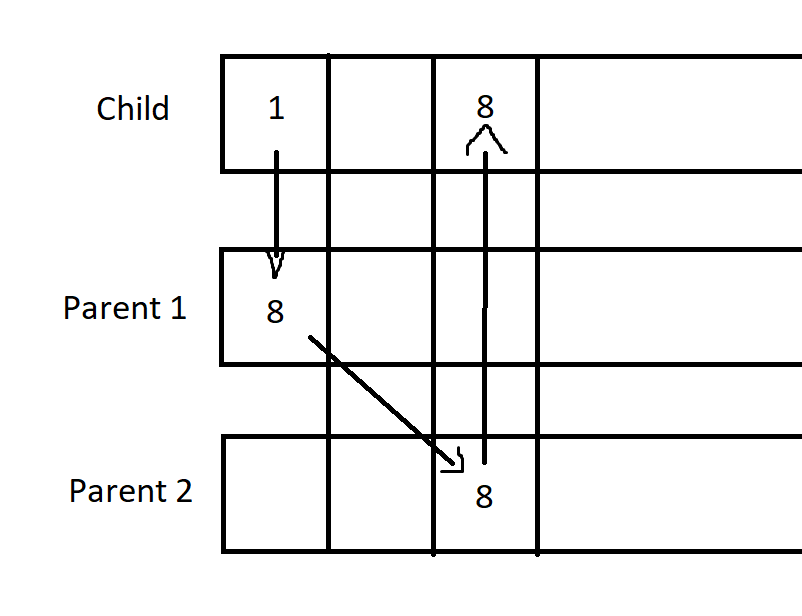
\includegraphics[width=0.25\textwidth]{CXExample}
\end{wrapfigure} 
This repeats until the we form a loop, when this happens we fill the remaining blank positions with the bits of those positions from the other parent. This is similar for the second child but the roles of the parents are reversed.\\\\The order crossover (\cite{crossover}) works by finding two random cut points which split the list into three sections. The middle section of each parent is then copied to the middle section of each respective child. Next, the cities are copied into the child from the opposite parent in order, after the second split index, excluding any cities already in the target child from the first step. This is repeated for the second child and then the children are returned.\\\\
The Genetic Algorithm itself works as follows:
\begin{itemize}
	\item It reads the name of the city, the distance matrix, and the size of the city(number of cities) using the readFile function. Then, a tours list and an initial tour list is instantiated.
	\item Makes the initial tour by appending 0-(size-1) to the initial tour list.
	\item The algorithm then sorts the initial tour into a random order.
	\item For each tour, the value in the first position is appended to the end to get a valid tour.
	\item Each new tour is appended to the tours list.
	\item Once we have created the initial population, we calculate the fitness of the population by getting the tour size of each member.
	\item The number of breeding pairs (n) is calculated by doing the floor function of the population size multiplied by the breeding probability, and multiplying by 2.
	\item The indices of each prospective parent are selected; the n fittest are selected.
	\item These n fittest(where n\%2 = 0 for all n) are divided into couples.
	\item For each set of couples, the crossover function produces two children which are appended to a list named ``children". At this point, once the children have been produced, there is a small probability that one, or both, of the children will mutate. This means that two random cities in the tour will switch places.
	\item Then we do some local optimization; if the tour has more than 4 consecutive cities in order, this subset is reversed.
	\item We then make use of a principle called elitism. This is when, with some probability, the fittest parent is carried through to the next generation.
	\item The list ``tours" is set equal to children, and this process repeats for the number of generations.
	\item Finally, the algorithm returns the minimum of the children, along with the tour produced.
	\item This data is placed into the requisite tour file in the format specified.
\end{itemize}
\subsection{Simulated Annealing Algorithm for TSP (B)}
The Simulated Annealing Algorithm has three parameters; the temperature, the number of iterations, and the amount to lower the temperature by each iteration. It makes use of a getDist function which returns the length of a tour, and a readFile function to read in a distance matrix for the graph from a file. I experimented with how to move to a neighbouring tour for quite a while; I thought one could be reversing a sub-tour of the tour. Eventually, I defined the notion that a neighbour is the same tour, but with two of the cities swapped. Another thing that I changed with the simulated annealing algorithm is the the cooling factor. This was originally just linear which produced results which were far from optimal. I changed this to exponential, logarithmic, and finally a non-monotonic adaptive cooling factor. The exponential cooling method $t_k= t_0 \cdot \alpha^k$(\cite{cooling}) worked better than the linear cooling method but there was still room to improve. Next, I tried a logarithmic cooling method, this worked very well; I used $t_k= t_0/(1+\log(1+count))$(\cite{cooling}). The method that I finally settled on as getting the best results in practice was the non-monotonic adaptive cooling which cools the temperature each iteration based on the best result and the last result in the function: $t_k = t_k \cdot (1+(f_{si}-f^*)/f_{si})$ (\cite{cooling})where $f^*$ is the best tour distance at that moment, and $f_{si}$ is the most recent tour distance. Also, I attempted to improve upon this by making a monotonic inverse quadratic cooling method along with a neighbour of the current tour being the same but with a random subset of the tour reversed. This was better than linear and exponential but was not the best in practice. Also, the added complexity of the derivation of a neighbouring tour meant that the time taken to compute the tours was much greater. Not to the point that it became impractical but definitely not worth the hit to the time taken.
The Simulated Annealing Algorithm works as follows:
\begin{itemize}
	\item It reads the name of the city, the distance matrix, and the size of the city(number of cities) using the readFile function and then instantiates an initial tour list.
	\item Makes the initial tour by appending 0-(size-1) to the initial tour list
	\item It finally appends the city at the start of the tour to the end to make it a valid tour, and appends to the tours list.
	\item Next, the accepting threshold is calculated using the cooling methods above; this is the amount over the current tour's distance which would result in the new tour being accepted.
	\item Two random indices are computed to be swapped; we ensure that these are not equal and once we have two unique indices we swap them. If this is the first or last item then the other one is changed to make the tour valid.
	\item We make the initTour equal to the neighbour if its distance is less than the original tour, or is within the accepting threshold over the original tour. This accepting threshold is defined by the temperature at each iteration.
	\item This is repeated for the number of iterations and the temperature is changed by some amount each time; this depends on the cooling method which is being implemented. 
	\item The methods which I experimented with have been detailed above. This means that the acceptingThreshold also changes (generally gets lower) every iteration.
\end{itemize}
\section{Results}
In this section I will focus on the results produced by my algorithms for inputs of varying length (Ranging from length 12 to length 535). I will also vary the parameters of each algorithm respectively to attempt to produce the best results. For the genetic algorithm, this will be about how altering the breeding probability, mutation probability, and initial population size over some number of generations affected the results achieved by the algorithm. \\\\
For the simulated annealing algorithm, this will involve talking about how varying the initial temperature, number of iterations actually, and cooling method affected the results achieved for the tours. \\

\begin{center}
\begin{tabular}{|c|c|c|c|c|}
\hline
Algorithm & Size & Time For 1 Execution/s & Best Tour Length & Average Length Over 10 Executions\\
\hline
Genetic (A) & 12 & 1.78 & 56 & 60.2\\
\hline
 & 17 & 2.79 & 1756 & 1951.3\\
 \hline
 & 21 & 3.27 & 3040 & 3486.9\\
 \hline
 & 26 & 3.23 & 1654 & 1758.2\\
 \hline
 & 42 & 4.78 & 1521 & 1868.0\\
 \hline
 & 48 & 5.12 & 20783 & 27281.5\\
 \hline
 & 58 & 5.74 & 49143 & 75667.5\\
 \hline
 & 175 & 16.08 & 39075 & 43241.3\\
 \hline
 & 180 & 19.29 & 421080 & 544343.0\\
 \hline 
 & 535 & 59.80 & 129019 & 142803.2\\
 \hline
Simulated Annealing (B) & 12 & 1.01 & 56 & 79.6\\
\hline
 & 17 & 1.40 & 1831 & 1869.5\\
 \hline
 & 21 & 1.49 & 2845 & 3578.5\\
 \hline
 & 26 & 1.90 & 1606 & 1688.9\\
 \hline
 & 42 & 2.93 & 1246 & 1355.2\\
 \hline
 & 48 & 3.49 & 15693 & 17919.5\\
 \hline
 & 58 & 4.32 & 33738 & 40331.8\\
 \hline
 & 175 & 9.57 & 26323 & 27203.3\\
 \hline
 & 180 & 9.47 & 14840 & 20126.0\\
 \hline 
 & 535 & 30.10 & 74660 & 77595.4\\
 \hline
\end{tabular}
\end{center}
For the genetic algorithm, I experimented with different types of crossover (\cite{crossover}). The first one as mentioned was the simple, split in the middle and swap the former and latter halves of each tour. This produced quite poor results for the majority of the graphs, of varying sizes. The next one I tried was the cycle crossover operator which I would have assumed to produce the best results, however, for the majority of the graphs this was not the case. The crossover method that I finally ended up using was the order crossover operator which produced the best results by far for the majority of the tours in practice. The parameters for the genetic algorithm were the mutation probability, breeding probability, number of generations, the initial population, and I also experimented with a thing called elitism. The best results came when the mutation probability was low and breeding probability was medium to high. This meant that the values focused in on a value and didn't vary much towards the end. Obviously, the number of generations was directly proportional to the performance; the higher the number of generations, the lower the tour length. This is obvious because there is more generations for improvements towards the minima. The higher the initial population the lower the final tour length: it meant that there were simply more tours to breed together. Elitism is when there is a probability that the fittest parent will be passed onto the next generation alongside offspring. I found that the higher the chance of this the better the results were because if by some bad luck the children produced were not as good as one of the parents, this good tour would not be lost. For this algorithm the results I achieved were varied. For the smaller size cities the tours produced seemed to be much better; getting close to optimal for 12,17, and 21. As the size increased the results became less good but still passable when taking into account the small amount of time it takes to compute the tours. As can be seen from the table, the averages are, for the most part, relatively close to the best tour length achieved. This shows that the algorithm is somewhat consistent whenever it is executed.\\\\
For the simulated annealing algorithm, I experimented a lot with different cooling methods (\cite{cooling}). The cooling method which I used during my initial implementation was a linear one. This was not good at all and produced awful results; this is because it is best to have a temperature drop off which is large to begin with and smaller later on, as I have now learned. The next one I tried was exponential temperature cooling which was much better than the linear cooling just based on the shape of the function. This was beaten by the logarithmic cooling method by a considerable amount. I also made use of the inverse quadratic cooling method with an alternative neighbour derivation, but this was not as good in practice as the non-monotonic adaptive cooling method which is what I have used. The parameters for the simulated annealing algorithm were the initial temperature and the number of iterations. I found that the best results came from high initial temperature and high number of iterations. This is because the initial high temperature means that in the first few iterations the accepting threshold will be rather high. With the cooling methods described (apart from linear) this drops quite quickly. This means that the values quickly approach a minima. As can be seen from the simulated annealing algorithms results, this algorithm is consistently better than the genetic algorithm. It produces better tours for all but one of the city sizes, and does better on average for all of the city sizes except for size 12. We can also see that the algorithm does this in much less time than the genetic algorithm; for a city of size 535 it almost halves the running time needed.\\\\
\bibliography{bibfile}


\end{document}